
\begin{savequote}[8cm]

  \qauthor{}
\end{savequote}


\chapter{\label{chap:researchSetting}Research Setting}


\minitoc




                                  \begin{CJK}{UTF8}{gbsn}


%\section{The Temple of the God of Agriculture Sports Institute}
I first visited the Beijing Temple of the God of Agriculture Sports Technology Institute (\textit{Beijingshi xiannongtan tiyujishu yundong xuexiao} 北京市先农坛体育技术运动学校,
hereafter the Institute) first thing in the morning on my first Monday in Beijing.  I entered via the main entrance in the south and made my way west to the main administration building by hugging the southwest perimeter of the 30,000 seat capacity, multi-purpose sport stadium that dominates the Institute's campus (see Figure~\ref{fig:beijingXNT}). My aim that morning was to confirm the details of my proposed research with the vice principal of the Institute responsible, as well as the head coach of the rugby program.

I knew both the vice principal and the head coach from time spent in China studying (2006 and 2008) and coaching rugby (2013) prior to my doctoral research.  Although I had already received positive responses from both during the planning stages of my research, I still needed to confirm arrangements for research face-to-face.

When I announced to friends within the Chinese rugby community in Beijing that I was preparing to conduct research with the Beijing rugby team at the Institute, I received mixed reactions.  Those reasonably well acquainted with the politics of rugby in China, rugby in Beijing, or sport in China more generally, warned me about becoming too involved.  Perhaps they were worried that I might suffer a similar fate to the group of Beijing athletes and coaches involved in rugby's first appearance in the National Games in 2013 (explained in detail in Section ~\ref{sect:rugbyInChina}).  Adrian, for example, warned me to be careful, citing that the Institute was riddled with ghosts: ``There really are ghosts there, I'm telling you Lijie, you should keep your distance'' (真的有鬼啊,我告诉你李杰,你最好离远点吧).\footnote{Lijie (李杰) is my Chinese name.}  I naturally scoffed at these warnings, which were admittedly tongue-in-cheek.  I was, however, intrigued to learn more about the cultural, political, and psychological---as well as ancient cosmological---principles that lay beneath the recent history of the Institute.

The Institute is located in the heart of Beijing, just to the west of Yongding gate on the South 2nd Ring Road. As one can imagine given Beijing's 3000-year history, the centrally located land on which the Institute sits was not always home to sport facilities and professional athletes.  The Institute takes its name from the temple that was built on the land during the Ming Dynasty in the 15th century.  Yongding gate marks the southern end of the city's ancient north-south axis, which also includes, from south to north: Tiananmen Square, the Forbidden City, Jingshan Park, and the Drum and Bell Towers (see Figure ~\ref{fig:beijingTemplesXNT}).  For thousands of years, Chinese cities have been laid out on a north-south axis according to the principles of feng shui. The auspicious power or energy (\textit{qi} 气) of each monument along this axis is believed to flow upward from the south (south being the most auspicious and therefore important of the Four Directions in Chinese cosmology).

In addition to this spatial dimension of cosmological order, dynastic powers also sought to reinforce order temporally, through regular performances of ceremonial sacrifices.  In the Ming and Qing Dynasties, Emperors (or their commissioned representatives) used the Temple of the God of Agriculture (hereafter the Temple of Agriculture) during the middle month of Autumn and Spring (according to the Chinese lunar calendar), to perform Middle Sacrifices (in a system of Grand, Middle and Common sacrifices) in honour of the Harvest (\textit{nong} 农)---one of the four main cosmological principles, in addition to Heaven (\textit{tian} 天), Earth (\textit{di} 地), and Ancestors \citep[\textit{zu} 祖; see][98]{Brownell2008}.  However, when the Qing Dynasty (1644---1912) finally buckled under the pressure of Western Imperial occupation and popular revolutionary political movements in 1912, Confucian Sacrifices in Beijing's various temples ceased.

But as one form of ritual expired in China, another form began.
The embrace of the practice and spectacle of modern sport by the Republic of China (ROC, 1912---1948) and the People's Republic of China (PRC, 1949---present) has been so resounding and fundamental that sport stadiums (and the sporting events for which these stadiums were specifically constructed) have supplanted ancient temples and rites along Beijing's sacred north-south axis as a medium of communicating state order \citep{Brownell1995}.  The flow of auspicious cosmological energy in Beijing now begins with the Institute (which was originally founded in 1930) in the south, and ends 21km to the north where the National Stadium, National Aquatic Centre, and the Olympic Green---the iconic monuments of the Beijing 2008 Summer Olympics---are situated.  Since re-joining the International Olympic Committee in 1979, China's athletes have participated at every Summer and Winter Olympics (except for the 1980 Moscow Summer Olympics, for which China joined 65 other nations in boycott following the Soviet Union's invasion of Afghanistan in 1979), winning over 600 medals in 28 different sports.  China's performance on the international stage has been facilitated by a now enormous state-sponsored competitive sport system (\textit{jingji tiyu tizhi} 竞技体育体制), which consists of thousands of sport programs housed in secondary and tertiary level education institutions and specialist sport institutes throughout China's 34 provincial level regions.  According to China's National Bureau of Statistics, in 2016 China's sport industry reached a total scale of RMB 1.9 trillion yuan (USD300 billion).  Since 2014, when the central government first declared plans for sport to become a ``pillar industry'' of China's modern economy, the sport industry has been growing by an average of 18.2\% per year.  The central government has set a target total scale of 5 trillion yuan (USD800 billion) or 2\% of GDP by 2025.\footnote{For comparison, in 2016 the scale of the US sport industry was USD400 billion. At present, the Chinese sport industry is dominated by manufacturing (sport equipment, apparel, etc).  There is therefore considerable room in the Chinese sport sector for much higher value inputs, such as the development of the sports services (tournaments, leagues, activities).}

The Temple of the God of Agriculture first became associated with sport in the form of a horse-racing track at the southern gate of the Temple at the end of the Qing dynasty. But, even beginning in this period of history, not all of the energy that flowed from the sacred temple has been auspicious.  As I will explain below, the arrival of rugby to the Institute has been a predominant source of much of the most recent political and cosmological turbulence.  In brief, I entered the Institute almost two years after its rugby program had experienced a dramatic fall from grace following a publicly humiliating controversy that unfolded at the National Games in 2013.  Although I was personally captivated by the fact that the Institute was located in such a culturally meaningful location in Beijing, I was also slightly apprehensive about the potential state in which I was entering the rugby program and the Institute.

It was with a slight pang of nervousness, therefore, that I made my way from the southern gate, around the stadium, and towards the main office building to meet the Institute's vice principal.

\begin{figure}[htbp]
  \centering
  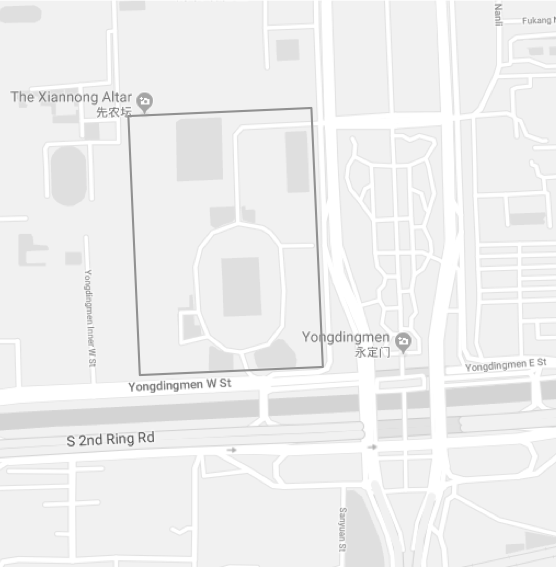
\includegraphics[scale =.5]{images/beijingXNT.png}
  \caption{Location of the Temple of the God of Agriculture Sports Technology Institute  (Source: Google Maps).}
  \label{fig:beijingXNT}
\end{figure}


\begin{figure}[htbp]
    \centering
  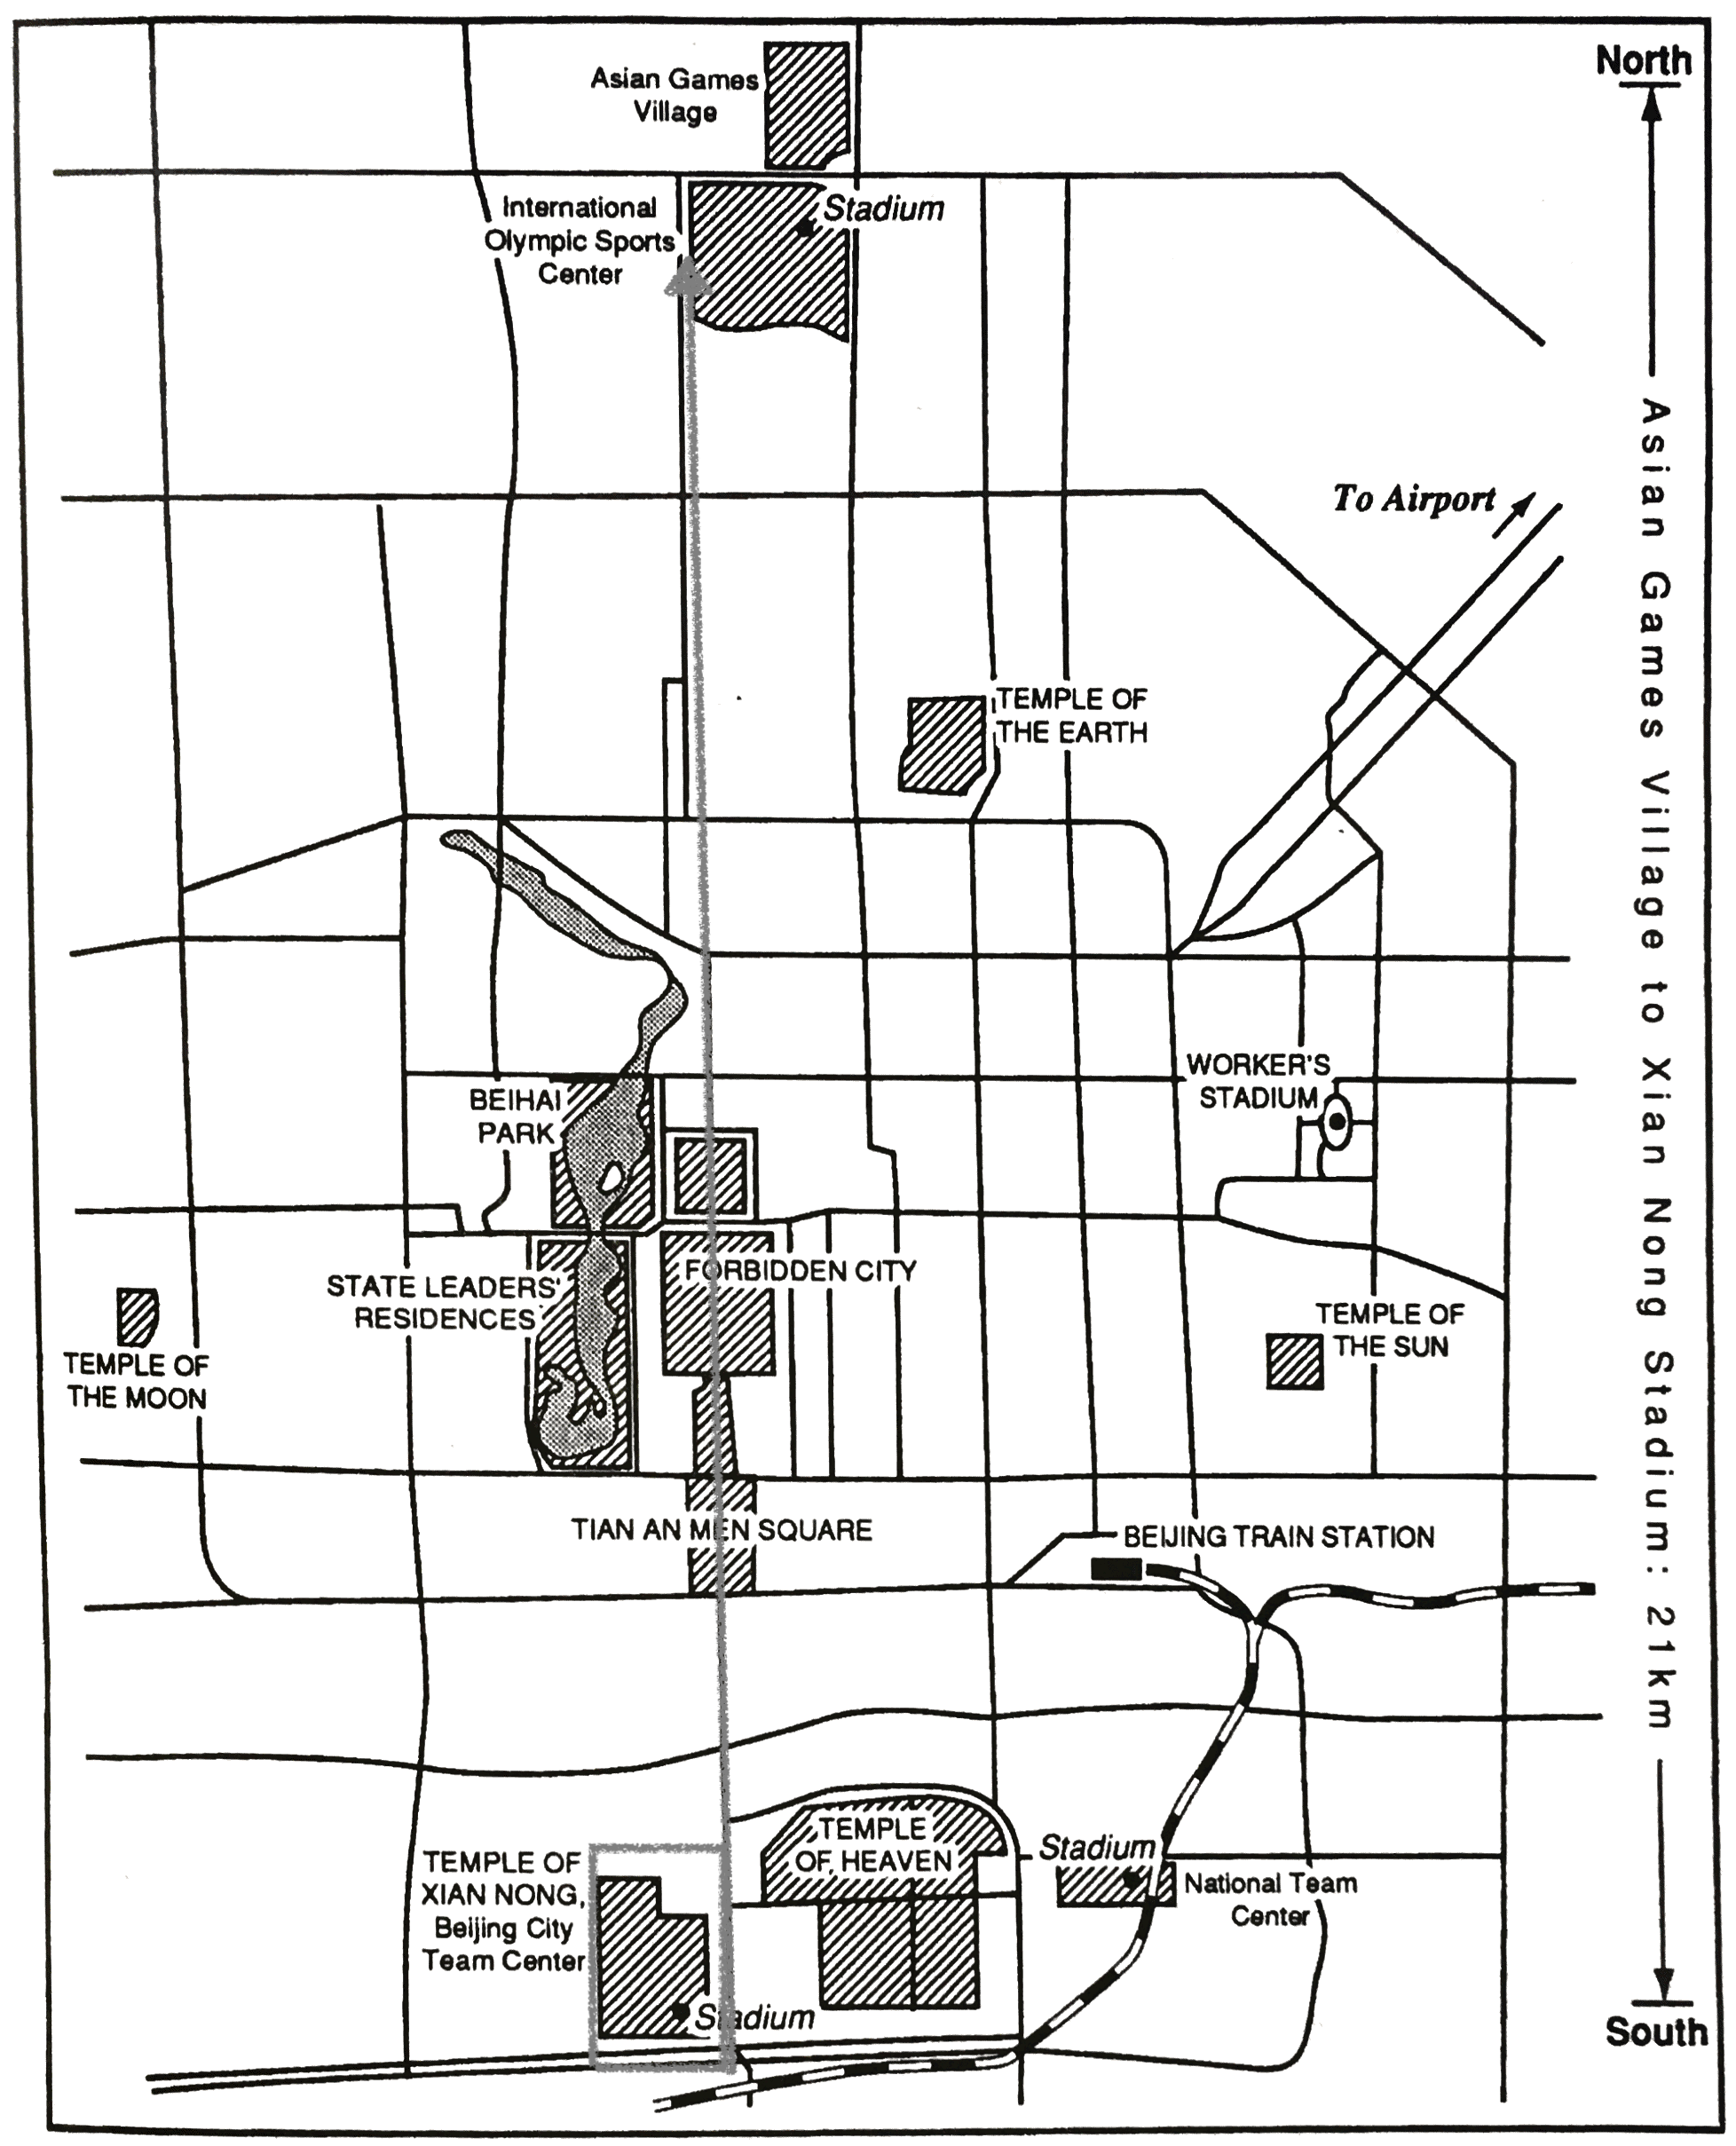
\includegraphics[scale =.1]{images/beijingTemplesXNT.png}
  \caption{Locations of former Qing dynasty temples and modern sport stadiums along Beijing's sacred north-south axis (Brownell 2008).}
  \label{fig:beijingTemplesXNT}
\end{figure}

%width = \linewidth,


\section{Introduction}
In this chapter, I introduce the empirical research setting in which I test a general theoretical account of team click in group exercise.  I introduce three core layers of context in order to situate a general theory of team click in the context of rugby in China.  The first and most immediate layer pertains to the specific parameters of joint action prescribed by rugby union.  The second layer pertains to the cultural system in which rugby is enmeshed: contemporary China. The third relates to rugby's specific history in China.

In this thesis, I do not attempt to explicitly address the question of how variation according to activity or culture alters hypothesised relationships between joint action, team click, and social bonding.  Rather, I seek to situate general theoretical claims within a specific group exercise setting, so that these claims can be meaningfully tested.  A general account of team click in group exercise hinges on the proposal that, in joint action involving higher levels of uncertainty, perceptions of higher levels of success in joint action, higher levels of team click, and higher levels of social bonding, will arise from higher levels of coordination of a) physical movement and b) social communication (see Section ~\ref{}). Thus, before progressing straight to an assessment of the research hypotheses of this thesis in light of empirical data,  it is crucial to first comprehend both a) the parameters for physical movement and b) the modes of social communication in that constitute a particular real-world group exercise setting.

An introduction to these layers of context---rugby, China, and rugby in China specifically---helps identify what patterns of physical movement (owing to the prescribed parameters of rugby) and what aspects of social communication (owing to the cultural context of China) will be \textit{shared} between co-actors in joint action.  I consider the the three layers of context from a dynamical perspective as cultural affordances that serve to reduce uncertainty in social interaction \citep{Ramstead2016}.  Evidence suggests that shared knowledge between co-actors in joint action may function as a  ``coordination smoother'' \citep{Vesper2017}, which serves to reduce the uncertainty of joint action by enabling higher levels of coordination of physical movement and social communication.  Thus, introduction to the core layers of context of the research setting will help render the processes that facilitate team click in group exercise in terms of the cultural affordances specific to rugby in China.

Rugby union is an interactive, field-based team sport that requires of its participants high levels of uncertainty owing to complex, socially coordinated movement and extreme levels of physiological exertion.  In addition, rugby is anecdotally and colloquially associated with social bonding in many of the contexts in which it is commonly played \citep{Dunning2005}.  The combination of highly complex and physiologically costly joint action demands, and anecdotally observable social effects makes rugby union an ideal arena to investigate the predicted explanatory role of team click in a theory of social bonding through joint action (Research Hypothesis 1).

Studying the sport of rugby in a non-traditional rugby playing nation like China creates a unique opportunity to assess the hypothesised role of uncertainty in joint action on team click and social bonding (Research Hypothesis 2). High levels of natural variation in familiarity with the technical requirements of rugby union, particularly among the members of the Beijing men's team (ethnographic study), meant that I was able to investigate the role of varying levels of uncertainty on experiences of joint action, including perceptions of team performance, team click, and social bonding.

The cultural milieu of China will also reliably shape patterns of experience and expression of joint action.  Numerous strands of psychological and anthropological research have converged on the proposal that cultural systems can shape patterns of attention and behaviour in non-negligible ways.  With the longest continuous cultural history in the world, China boasts a rich and diverse terrain of cultural affordances that are of potential relevance to culturally specific patterns of experience in joint action.  Of most relevance to this thesis is the proposal that the cultural context of contemporary China (broadly construed) facilitates a \textit{relational} mode of social cognition \citep{Nisbett2003,Yuki2005}.  As I outline in more detail below, a mode of social cognition refers to the way in which a specific field of cultural affordances reliably shape patterns of action and perception, self-construal, group formation, and institutional norms \citep{Nisbett2003a}.

Specifically, evidence from anthropology and cultural psychology suggests that a relational (as opposed to categorical) mode of social cognition will encourage emphasis on holistic (over logical) reasoning, attention to and maintenance of particularistic (and hierarchically organised) social relationships (over deontological commitments to categorical social identities such as self, group, or nation), and an ethic of personal cultivation in group membership \citep[over an ethic of self-less egalitarianism; see][]{Liu2009}.  While I do not expect variation in modes of social cognition to fundamentally alter hypothesised relationships between uncertainty, perceptions of team performance, team click, or social bonding, I do expect these relational processes to bear upon Chinese rugby player's experience of joint action. Research suggests that the joint action demands of rugby and the cultural context of China will pattern modes of action and perception in joint action, expressions of group membership to the team, as well as broader socio-institutional processes in which athletes are embedded.

In the sections that follow, I situate a general account of team click in group exercise by accounting for the cultural affordances that will reliably shape and pattern athlete experiences of joint action.  I begin by introducing the research setting of rugby in China and my research methods (Section ~\ref{sect:researchSettingMethod}), before presenting theoretical and ethnographic evidence for the way in which the physical and social demands of rugby and a dominant relational mode of cognition bears upon athlete experience of joint action in group exercise.



%Further, my ability as a researcher to identify relevant variables relevant to a general account of team click in group exercise will hinge on




%I expect high levels of uncertainty rugby's joint action to generate high levels of social bonding when joint action clicks.

%Specifically, high levels of uncertainty (owing to its complexity, intensity, and competitiveness) and interdependence (due to the fact that almost all action in rugby is joint action) in rugby makes rugby an activity particularly well suited to testing theoretical claims regarding the mechanisms of uncertainty and positive expectation violation that are hypothesised to underly the joint action --- social bonding link (Hypothesis 2).

%--both factors are known to be linked to social bonding \citep{Cohen2017,Davis2015}.

\section{The cultural affordances of rugby and China}


In this section, I outline the ways in which the specific technical and social requirements of rugby's joint action and the cultural context of China---namely, a dominant relational mode of social cognition---bear upon a general account of team click in group exercise.  In so doing, I generate expectations concerning athletes will experience team click and social bonding (Hypothesis 1) as well as uncertainty and expectation violation (Hypothesis 2) in joint action.

In short, high levels of uncertainty and interdependence associated with joint action in rugby I expect athletes to experience higher levels of uncertainty as more challenging, and instances in which uncertainty in joint action is reduced as more rewarding.  In addition, high levels of on- and off-field interdependence will make team identity and

, combined with high levels of variance in levels of athlete technical competence at the Beijing men's,

joint action as both technically and socially challenging and rewarding (in instances of successful performance).


Considering in particular most athletes' relative unfamiliarity of rugby's joint action


 Rugby: uncertainty in GE, interdependence and coordination requirements.

China: Experience of JA will be patterned by a relational mode of social cognition






\subsection{Rugby\label{sect:rugbyUnion}}

Joint action in rugby is defined by high levels of uncertainty and, relatedly, high levels of coordination of on-field movement and off-field social communication between co-actors.  This evidence is consistent with predictions informed by the AIF, that under conditions of higher uncertainty, more successful joint action will necessitate higher levels of coordination of physical movement and social communication.  Thus, rugby offers a suitable real-world context in which to investigate and assess a general account of team click in group exercise.  In this section I review existing evidence for uncertainty and physical and social coordination in rugby union.

The diversity of technical demands in joint action make it a highly uncertain group exercise setting.  Rugby’s joint action demands a diverse and varied set of technical skills (involving numerous co-actors, sensory modalities, and spatio-temporal scales) be executed on-line and in the moment.  Rugby players run with the ball, pass or kick the ball to other attackers or towards open space on the field, enter collisions as either ball-carrier, tackler, or support player, and contest possession of the ball by grappling in ``rucks'' and ``mauls'' \citep{Ross2015a}.\footnote{In distinction to American Football (NFL), in rugby only the defensive team is only permitted to tackle the the ball-carrier from the attacking team.}  Like many equivalent team sports in which a single ball (or similar object) is contested, such as basketball, association football, and ice hockey, game play in rugby typically involves a series of sub-phases in which attacking and defending subunits of athletes contest possession of the ball \citep{Passos2011}.  Athletes commit to multiple hierarchically nested goals---some of which they share with the entire field of athletes (for example, the shared goal of playing a game, or adhering to the rules of rugby), while other goals they share only with their own teammates (e.g., winning the game, controlling possession of the ball), or with a select subset of their teammates (e.g., coordinating with a teammate in attack to outsmart the defence).  In addition, the competition between teams in rugby will further increase uncertainty, owing to the continual presence of attempts to foil and disrupt prediction, perception, and action. It is also possible that extremely high levels of physiological exertion characteristic of rugby could have indirect implications for cognitive function \citep{Dietrich2004a}.  All these factors considered together from the perspective of uncertainty suggests that rugby's joint action will be highly uncertain.  It can therefore be expected that athletes who adhere to rugby---particularly for individuals or teams whose familiarity with rugby’s joint action is relatively low---will experience joint action as challenging, owing to high levels of uncertainty in rugby's joint action.

For rugby players in China in particular, it is even more likely that high levels of uncertainty in joint action will pose high technical challenges, owing to the sport's minnow status within the Chinese sports system (explained in Section ~\ref{sect:rugbyInChina}).  Most professional rugby players in China either start from scratch with sport when they arrive at rugby programs as young adults, or else transition to rugby start from an individual sport (such as athletics) defined by lower levels of joint action uncertainty.


\subsection{Coordination}
In line with the predictions of the AIF outlined in the previous chapter, it can be expected that higher levels of uncertainty in rugby's joint action will demand higher levels of coordination of physical movement and social communication in order to be perceived as more successful.  Existing evidence surrounding the sport of rugby supports this suggestion: rugby’s on-field demands clearly demand high levels of coordination in order for joint action to be performed successfully, and there is also existing evidence to suggest that rugby is associated with processes characteristic of social bonding.

\subsubsection{On-field coordination}
In the case of rugby, all action is joint action.  The performance of almost all technical actions require either direct or indirect consideration of the position and intentions of other athletes in relation to that action \citep{Downey2012}.  Even the most seemingly independent technical operation among these skills---for example, an athlete kicking the rugby ball to open space on the field---requires the consideration of positioning of other athletes.  Joint action in rugby is therefore defined by high levels of on-field interdependence.

Because all action is joint action in rugby, it is hard to delineate perceptions joint action from individual action.  Instead, I characterise joint action in terms of its individual-level and team-level perceptions of performance. Perceptions of team performance may include the development of an impression of how the team (or a specific subunit of the team) is managing to coordinate the defensive or attacking line, or how well the team is communicating throughout a game, or supporting each other in attack and defence.  Perceptions of individual performance, by contrast, may involve athlete perceptions of their individual-level contributions to attack, such as the quality of their passing technique, or their positioning as ball-receiver, or their ability to make effective decisions.  In defence, athletes may attend individual level performance such as one-on-one tackling performance, or effectiveness in contesting possession in rucks or mauls (effectiveness in the ``contact'' area).  In this sense, one level of performance evaluation is more dominantly team-based, while the other is more dominantly individually-based.  Given that team click is an inherently team-level perception (see Chapter~\ref{sect:teamClickEmpirical}), I focus predominantly on perceptions of team performance success.


%Various contextual and individual-level factors may underpin variation variation in the extent to which individuals attend to either level of performance. role of uncertainty on confidence / expectations for team performance

\subsubsection{Social coordination}
Rugby also appears to generate experiences and perceptions characteristic of social bonding.  Rugby is a sport traditionally associated with the colloquial interpretation of ``social bonding,'' particularly in all-male social organisation common in the elite educational spaces of England and Commonwealth countries in which rugby originally developed \citep{Dunning2005,Richards2007,Collins2008}.\footnote{Recently, rugby union has been the site of much criticism due to the fact all-male social groups that cohere around the sport of rugby appear to support and sustain hyper-masculine and hyper-normative behaviours, including gender-related violence \citep{Cosslett2014}.}  Rugby is also a sport associated with social virtues.  ``Rugby is a game for barbarians played by gentlemen,'' or so the saying goes.\footnote{The origins of this oft-cited adage are unclear.  The phrase is supposedly the adopted motto of the British Barbarians Football Club, established in 1890 \citep[34]{Dunning2005}.  The complete phrase reads ``Rugby is a game for barbarians played by gentlemen, football is a game for gentlemen played by barbarians.''  However, official club history cites its original motto as, ‘Rugby Football is a game for gentlemen in all classes, but for no bad sportsman in any class' \citep[vii]{Starmer-Smith1977}.  Some sources attribute the saying to British writer and poet Oscar Wilde (1854-1900) \citep{Fleenor2015}}.
Different inflections on this adage have been reproduced by people in all parts of the world that rugby has reached, including China \citep[see][]{Taylor2010}).  Presumably, this saying has survived due to its ability to tether the nature of rugby's physical requirements with socially valorised moral virtues of fair play, cooperation, and integrity.  The current slogan of World Rugby (rugby's international governing body) is ``Building character since 1886,'' \citep{WorldRugby2017}.  This phrase was presumably chosen to draw an association between the joint action requirements of rugby and the moral and social character that can be generated through participation in rugby.

In sum, rugby will be highly suited to application of a general account of team click in joint exercise, due to the way in which the rugby appears to reliably generate uncertainty and demand physical and social coordination in joint action.  As predicted by the AIF, higher levels of uncertainty in joint action will demand high levels of coordination of physical movement and social communication for joint action to be successful.  This proposal serves as a foundation for Hypothesis 1 of this thesis, which states that higher levels of perceived success in joint action will predict higher levels of social bonding, mediated by team click.  In addition, high levels of uncertainty in rugby’s joint action will allow for the assessment of Hypothesis 2 of this thesis, which states that higher levels of team click will arise from a pathway involving two causal relationships: one between a) higher levels of uncertainty in joint action and lower levels of expectations surrounding team performance success (Hypothesis 2.1), and b) higher levels of positive expectation violation and team click (Hypothesis 2.3).

Based on these consideration of rugby’s physical and social joint action requirements, it can be expected that rugby's joint action, and team performance in particular, will entail high levels of uncertainty, and demand high levels of physical and social coordination in order for team performance in joint action to be successful.  Under these conditions, I expect that athletes will experience uncertainty in rugby’s joint action as a technical challenge that leads to social inferences.  Such inferences could include 1) low expectations for team performance (relative to individual performance), 2) stress and or anxiety concerning (pre performance or when performance fails), or 3) elation or positivity affect (when joint action is successful).  Coordination of physical movement and social communication should be identifiable in terms of experiences of interdependence on and off the field.

%In sum, rugby offers a suitable group exercise setting in which to situate and test a general account of team click in group exercise.  It is possible that the experience of higher levels of uncertainty in rugby's joint action will relate to higher levels of on-field coordination of physical movement and off-field coordination of social communication (in the form of processes characteristic of social bonding) when joint action is performed successfully.

%It can be expected that this underlying theoretical relationship between uncertainty and coordination posited by the AIF will bear upon athlete experience in a number of ways. Athletes may experience the uncertainty of joint action as challenging, or perceive success in on-field coordination in joint action as rewarding.

                %    * Coordinate social communication of challenge and reward in joint action performance, as well as their social experiences of group membership.


                %Thus, given that they are underwritten by this theoretical foundation (coordination of phys~soc),  the hypotheses of this thesis.





\subsection{China}
In this section, I introduce tenets of a Chinese relational mode of social social cognition, which evidence suggests will reliably shape and pattern experiences of joint action in contemporary China.  Specifically, relational processes of holistic reasoning about social relationships and dynamics, attention to particularistic, hierarchical networks of social relationship, and the social virtue of personal cultivation, will bear upon coordination of on-field physical movement and off-field social communication in group exercise contexts in contemporary China. Comprehending variation in modes of social cognition according to culture is an important prerequisite for situating a general account of team click in a real-world group exercise setting.  Recognition of variation in processes of social cognition allows for the accurate identification and interpretation of primary data, in this case pertaining to the experience of team click and social bonding in joint action.

A gradual accumulation of research across the human sciences suggests that cultural environments can reliably shape attention, perception, and action.  Anthropologists have for some time emphasised meaningful cultural variation in processes of social group formation \citep{Strodtbeck1961,Kluckhohn1961,Mead1967,Fei1992}, and cultural psychologists have sought to demonstrate this variation in experimental paradigms \citep{Markus1991,Nisbett2001}.  More recently, various strands of ``indigenous'' psychology \citep[e.g., Chinese indigenous psychology, see ][]{Liu2009}, have sought to compliment cultural psychology---which largely seeks to test variation in psychological processes between different cultural systems---by attempting to account also for variation within cultures.  Together, this research offers a framework that allows for a scientific description of the various cultural affordances that may reliably shape and pattern experiences of joint action in contemporary China.

A core finding from cross-cultural psychology concerns the correlation between cultural variation and modes of and group formation.  Current research suggests a theoretical spectrum of processes of group membership, the two poles of which are usually described as ``categorical'' and ``relational'' \citep{Hofstede1980,Brewer2007}.
In the case of some cultural niches, traditionally samples from modern and industrialised ``Western'' societies (such as the USA), social identity formation revolves around the autonomy and immutability of social categories of ``self'' and ``group.''  By contrast, in societies in which a ``relational'' mode is dominant (for example, in East Asian countries such as Japan, China, Korea, etc.), social identity is defined primarily according to degrees of social embeddedness and interdependence with others comprising their in-groups\citep{Leung2012}.

A considerable amount of evidence has amassed within cultural and social psychology to suggest that the existence of meaningful contrasts between samples of East Asian populations (predominantly undergraduate students of Japanese, Chinese, and South Korean universities) and Western populations (predominantly undergraduate students of North American and Western European universities) in domains of attention and perception \citep{Peng1997,Nisbett2003}, psychological construal of social categories of self and group \citep{Markus1991}, behavioural tendencies in social interaction \citep{Yuki2003}, and institutional norms \citep{Liu2017}.
Modes of group membership have been shown to vary not only across cultures (i.e., East Asian versus Western European or North American), but also within cultures \citep{Henrich2014}, within social groups \citep[according to sex and personality differences, see][]{Yuki2014}, and even within individuals \citep[depending on contextual and situational primes, see][]{Lee2014,Wong2005}.  The prominence of one mode of membership over another in broad ethnic or cultural groups (e.g., The West versus East Asia) appears to be associated with the durable persistence of cultural and linguistic institutions that afford particular patterns of social cognition. Thus, while broad cultural modes of social cognition are not understood to be hard-wired, it can be expected that distinct cultural trajectories will enable the production and transmission of reliable patterns of social cognition over others \citep{Claidiere2014,Mesoudi2015}.

Divergent modes of social cognition appear to reliably preference different psychological mechanisms for processes of group membership and social self-construal.  The canonical ``social identification'' paradigm, of social psychology, for example, requires that an individual make an identification between abstract categories of the self and the in-group or out-group \citep{Turner1987}. Group membership is achieved when the perceived differences between the self and other in-group members are smaller than the perceived differences between in-group and out-group members \citep{Yuki2014}. Categories of self, other, and group are construed constructs that reliably moor an individual's perception of personal and social identity.  This proposal forms the basis of many validated psychological constructs used by social and evolutionary psychologists to measure social bonding and affiliation between individuals and between individuals and the group \citep{Swann2009,Wolf2015}.  Thus, there is a general persuasion in social and evolutionary psychology to conceive of (and measure) social processes group membership and social bonding in terms of categorical social identity \citep{Liu2015a}.

%Categorical modes of social cognition have formed the foundation of Anglo-American social psychology of the 20th Century, thus occupying a hegemonic position for understanding how humans cohere socially \citep{Liu2005}.

In distinction to categorical modes of social cognition, relational mode of social cognition predict that individuals attend more predominantly to maintaining and harmonising intra-group relationships, rather than engaging in intergroup categorical comparisons to substantiate individual psychological reality \citep{Yuki2003}.  In a relational mode of group membership, social identity derives less from a calculation of psychological distance between abstract categories of self and in-group, and more from a degree of commitment to cultivating a network of hierarchically structured---but more or less self-centred and self-enhancing---relationships \citep{Liu2009,Nisbett2003}.

It has been shown experimentally that categorical group processes facilitate fast and effective identification with arbitrary minimal groups \citep{Diehl1990,VanBavel2014}, arousal of intrapersonal cognitive dissonance between the self and experimentally constructed in-group \citep{Festinger1957,Stone2001}, higher levels of cooperation with categorically similar strangers in economic games \citep{Yuki2005,Yuki2003}, and greater attention to and memory recall \citep{Buchan2006,Ng2016}.  By contrast, the inverse is usually observed in experiments where relational processes of group membership are made more prominent or salient.  It has been noted, for instance, that minimal group experimental paradigms have had very little (if any) success in East Asian (particularly Japanese) contexts \citep[586]{Liu2009}.  Instead, relational group processes appear to allow for the arousal of cognitive dissonance only when it is constructed interpersonally (as opposed to intra-personally) between an individual and specific individuals to which that individual is connected by a meaningful social relationship \citep{Hoshino-Browne2005}.  Likewise, individuals with predominantly relational group awareness are more willing to cooperate with and attend to strangers with whom they share relational rather than categorical ties \citep{Ng2016,Yuki2005}.

%E: Taken together, this evidence suggests that, in the case of joint action, divergent modes of group membership may serve to reliably shape

Understanding the cultural contours of social cognition in China requires an engagement not only with contemporary findings from cultural social psychology of group membership, but also with what social psychologist James Liu terms an ``indigenous Chinese psychology'' \citep{Triandis1996,Liu2009}.  Liu argues that theoretical generalisations based on evidence from cultural psychology alone runs the risk of being frail to the behavioural diversity observable both between the East Asian nations (Japan, China, Korea among others), and within each individual nation itself (for example, the vast internal cultural variation in China between North and South; East and West \citep[see, for example,][]{Henrich2014}).  To bolster claims of cultural psychology, Liu and colleagues suggest the utilisation of a ``representational'' account of social psychology \citep{Liu2005}, in which socially shared representations of history are central to creating, maintaining, and changing psychological identity and patterns of social interaction.  A representational account accords neatly with the definition of cultural affordances adopted herein.

Indigenous Chinese psychology locates tendencies for group membership within a specific historical trajectory of cultural processes.  In particular, it is generally agreed that contemporary China is the product of an ongoing interaction between two distinguishable historical processes: 1) two millennia of cultural continuity associated with the ancient development of a singularly successful, multilingual Chinese civilisation, and 2) a more recent engagement with---including, importantly, perceived sufferings and failings at the hands of, and hopes of rejuvenation within---global activities of commerce, governance, knowledge production, nation-building, and international relations \citep{Liu2009}.  In turn, these processes have given rise to three core representational (i.e., cultural) affordances of indigenous Chinese psychology: 1) ethically-prescribed Confucianism, 2) formidable legal and bureaucratic systems of state governance, and 3) modern Chinese nationalism, fuelled by representations of Marxist/Leninist dialectical materialism and revolutionary sprit, as well as faith in scientific and technological advancement \citep{Barme2009}.

Tenets of indigenous Chinese psychology can be combined with findings from cultural psychology to form three core processes of a distinctly Chinese relational mode of social cognition \citep{Liu2014}:

    \begin{enumerate}
      \item \textbf{Holistic reasoning} is commonly employed to represent and harmonise social relationships and avoid interpersonal conflict, via the principle of the  ``middle way'' \textit{zhongyong zhidao} 中庸之道).
       \item \textbf{Hierarchical relationism} acts as a guide for managing hierarchically organised familial and social networks, known as ``guanxi'' (\textit{guanxi} 关系).
       \item \textbf{Personal cultivation} is employed as a means of accumulating ethical virtue, or ``human heartedness'' (\textit{ren} 仁).
     \end{enumerate}

These three dimensions of Confucianism can be identified in cultural affordances that pervade all spaces of contemporary Chinese social life, and bear upon real-world processes of social interaction, including joint action typical of group exercise.

\myparagraph{Holistic reasoning}
The postulate of holistic reasoning is commonly employed to explain human social behaviour.  Holistic reasoning involves less emphasis on reason in the Western epistemological sense (i.e., the search for ultimate knowledge via reduction), and instead suggests that manifest and latent aspects of reality come in and out of being through an interaction between the ``Receptive'' (\textit{Yin} 阴) and ``Creative'' (\textit{Yang} 阳) principles inherent in the universe \citep{Leys1997}.  In the case of knowledge of social interaction, a dominant point of interest should not be unchanging human biology, but rather the dynamic and evolving patterns of family, groups, society, and culture \cite{Nisbett2003}.

\myparagraph{Hierarchical relationism}
Hierarchical relationism builds on the dialectical reasoning of holism to provide cues and directives for managing reciprocity and responsibility in particular kinship and extra-kin social relationships \citep[\textit{renqing} 人情][]{Maehr1980}.   In this system, the individual stands simultaneously in several different relationships with different people: as a junior in relation to parents and elders, and as a senior in relation to younger siblings, and students. While juniors are considered in Confucianism to owe their seniors reverence, seniors also have duties of benevolence and concern toward juniors. The Five Relationships are: 1) ruler to ruled, 2) father to son, 3) husband to wife, 4) elder brother to younger brother, and 5) friend to friend. Four of the five key relationships concern unequal hierarchical relationships, the only exception being friendship, in which reciprocity and respect is emphasised.  Notably, none of the prescriptions concern strangers.  Hierarchical relationism renders social interaction in strong contrast to the practical ethics dominant in Western Europe and North America, which blends Enlightenment philosophy and Christian values to emphasise egalitarian concerns such ``respect for thy neighbour'' and Good Samaritanism \citep{Liu2005}.

\myparagraph{Personal cultivation}
A common stereotype surrounding East Asian societies is that processes of group formation are highly ``communal.''  The emphasis within Confucianism of harmonising hierarchical relationships can easily lead to the assumption that, in East Asian societies, attention to the group takes precedence over attention to the individual self.

When explaining my research to interested non-expert observers, most would respond to my ``elevator pitch'' with generalisations about the communalism of Chinese society and how such factors would encourage higher levels of social bonding in group exercise.  This line of folk-reasoning, while potentially commensurate with some psychological and anthropological evidence deriving from modern Japan \citep{Kitayama2010a}, represents a common misconception of indigenous Chinese psychology that results from constructing a mutually exclusive individual-versus-group binary based on (Western) epistemological assumptions derived from categorical modes of social identification \citep{Tu1998}.  In other words, the to stereotype East Asian cultures as communal contains a categorical assumption: when individuals attend to the social category of the group, they do so at the expense of the category of the self.

In counter-distinction to this assumption, Confucian thought promotes cultivation of the personal self as central to accumulating social virtue (\textit{ren} 仁), and vice-versa \citep{Hwang2012}.
In this conception, acts of self-cultivation, rather than being interpreted as anti-social, are instead often celebrated as expressions of pro-sociality.  This is supported by experimental evidence that personal-cultivation arouses little or no dissonance between categories of self and group \citep{Suh2002}, because these categories are generally understood to be distributed or porous rather than fixed and immutable \citep{Nisbett2003}.  Thus, far from being a derogated act (as in the tall poppy syndrome common to cultural milieus such as Australia), in Confucianism, self-cultivation is understood as an appropriate and even ultimate path or ``way'' towards sagely transcendence \citep[106]{Hwang2012}, and has been valorised in styles of leadership and public conduct \citep{Farh2000,Cheng2004}.
  \footnote{Paternalistic leadership, defined as a ``a style that combines strong discipline and authority with fatherly benevolence and moral integrity couched in a personalistic atmosphere'' is an example of public conduct in which the self is promoted as a social vehicle \citep[91]{Cheng2004}.  Paternalistic leadership promotes an ethic in which the individual acts in a dignified manner, exhibiting high self-confidence, tight control of information, and an unwillingness to delegate authority.}
Thus, within a Chinese relational mode of social cognition, it can be expected that the self can serve as a useful vehicle for overt pro-social behaviour, without arousing conflict between other's interests.

\myparagraph{Implications of a Chinese relational mode of social cognition for joint action and group exercise}
It can be expected that these three interrelated processes will be identifiable and salient in the context of rugby in China.  Specifically, a Chinese relational mode of social cognition will entail holistic reasoning about, and hierarchical conceptions of social relationships and groups, and will tend to promote personal cultivation as an ethic of group membership.    Importantly, relational and categorical processes should be understood as co-existing tendencies.  In this sense, while social categories of team and in will be salient and functional in real-world instances of Chinese social cognition, it may be that a relational mode preferentially directs attention towards the cultivation of relationships as a social priority.  In brief, I expect a relational mode of social cognition to be identifiable in patterns of attention, group membership, and institutional norms.

 %In this scenario, the personal self exists as a node in a relational network to which that node is already always connected, as opposed to existing as an independent category defined socially in terms of distance between other categories such as the group.




 \section{Research setting and method\label{sect:researchSettingMethod}}
 I begin by providing an historical background to rugby in China and my ethnographic setting in particular.  The history of professional rugby in China is situated within a specific history of modern sport in China.  In brief, athletes who arrive at the Institute (and other institutions like it) are motivated primarily by the life-course opportunities that the rugby program at the Institute affords, namely tertiary education and future employment.

 Rugby is an interactional team sport played on a rectangular field (100m x 70m), by two teams of 15 players each, who contest possession of an egg-shaped ball that can be used to score points \citep{IRB2014}.  Descending from a variety of locally-specific folk games played in pre-industrial England, all loosely grouped as ``football,'' rugby developed within the elite public school system as a deliberate physical activity arbitrated by rules and regulations, before circulating through the arteries of Great Britain's colonial empire as a leisurely pastime—--a ``sport'' \citep{Dunning2005}.  In 1996, rugby became a professional sport and is played as such in Western Europe, the Southern hemisphere (Australia, New Zealand, South Africa, and Argentina), and Japan. Rugby sevens---the specific focus of this thesis---is a modified version of the conventional 15-a-side game involving teams of 7-a-side, and 14-minute games played in a Tournament structure over two or more days (rather than a one-off 80-minute match between two teams).  Rugby sevens has grown in popularity more recently, particularly since its introduction to the Olympics for the 2016 Games in Rio de Janeiro.  More so than the traditional version of the game, rugby sevens is played by countries all over the world, and attracts more balanced participation by men and women.

 As I explain below, in China, rugby is a minnow team sport---a ``cold gate'' (\textit{lengmen xiangmu} 冷门项目; a term that refers to a profession, trade or branch of learning that receives little attention)---with very little public recognition.  However, the recent inclusion of rugby in the Olympics (in its modified version of rugby sevens) means that there are now rugby programs throughout 10 of China's 34 Provincial level administrative regions.  The integration in China between the state-sponsored competitive sport system and secondary and tertiary education systems means that rugby programs are attractive to athletes not usually because of the fame, fortune, or honour of city, provincial, or national level representation that adherence to rugby could afford a professional rugby player elsewhere. Rather, athletes like Sun Hongwei arrive at the Institute motivated by the opportunity to attend a prestigious university, and thereafter to get a good job.

 While these explicit utilitarian motivations may be at the forefront of athletes' considerations when they first arrive at the Institute, and indeed persist in the background during their adherence to rugby, in my experience as a coach and researcher, the interdependence associated with rugby's on-field joint action and off-field social processes of group formation reliably captured the attention of almost all athletes who stayed for a period greater than merely a few weeks. In essence, many athletes experienced a transformation in which they became ``social creatures'' (as junior athlete Fang Chao commented to me), both on and off the field.


 \subsection{Sport in China}
 The emergence of modern sport and exercise in China is entangled with a history of interaction and conflict with, and embrace of foreign influence during the 19th, 20th, and 21st centuries.
 Prior to the introduction of Anglo-American interactional team sports and Northern European calisthenics (training exercises and gymnastics) in the late 19th century, physical activity that could be grouped in the broad category of sport and exercise was limited to a small collection of physical cultures indigenous to China, practices imported much earlier in history from south Asian religious traditions (e.g. Buddhism and Hinduism), and some activities imported from non-Han dynasties such as Manchurian horse racing in the Qing dynasty.  Historical records suggest that participation in almost all of these activities was limited to the imperial ruling classes and urban elites \citep{Ge2005}.

 Increased foreign imperial influence in China during the 19th century brought with it the introduction of an array of ideas and practices to China's urban elite ruling classes, including novel physical cultures of dress, adornment, leisure, and not least, physical exercise.  Sport first manifested in China in the promotion of Anglo-American competitive sports by North American Christian missionary organisations such as the Young Men's Christian Association (YMCA), and the incorporation of Northern European calisthenics routines into military exercises \citep[240]{Morris2004}.  Such techniques were soon popularised within elite intellectual communities as pedagogical tools designed to foster an explicit link between the strength of the physical body and the strength of the Chinese nation (\cites[32]{Morris2004}[49]{Brownell1995}).\footnote{The belief that sport and exercise were important pedagogical tools in the development of physically and mentally strong subjects of modernisation---an idea Increasingly popular at the time in Europe, North America, and Japan, \citep{Elias1986}---gelled with the values of a nationally (and internationally) motivated Chinese urban elite}

 \textit{Tiyu} (体育), the term in modern Chinese that most closely translates to sport, was one of many neologisms inherited from the Western social sciences via its Japanese translation \citep{Morris1998}.  Importantly, \textit{tiyu} encompasses more than just the modern Anglo-American competitive sports (roughly translatable to ``yundong'' (运动) that the English word connotes.  The modern Chinese concept of sport refers to an entire culture and discipline of the body that is deeply intertwined with the political project of Chinese modernisation and advancement \citep{Morris2004}.\footnote{As Lydia Liu (1995: 58) points out, even the notion of ``China'' itself as a term linked to a national imaginary, only began to emerge as such through interaction with Western missionary discourses concerning ``China'' during the 2nd half of the 19th century.}

 During the Republican Era (1912-1949), sport in China began to develop among urban elite along two main strands—--``competitive sports'' (\textit{jingji tiyu} 竞技体育) and ``games and calisthenics'' (\textit{ticao} 体操).  A significant aspect of competitive sports was the public spectacle of the ``games meets'' (\textit{yundonghui} 运动会), in which the performance of emerging national and international political identities could take place.  As early as 1908, the Chinese sport community enshrined the Modern Olympic Games (\textit{Aolinpike yundonghui} 奥林匹克运动会) as the pinnacle of participation in an international community of nations, and as such, the quadrennial global ritual has since preoccupied a collective Chinese sporting consciousness, and a Chinese national consciousness more broadly \citep{Jarvie2008,Barme2009,Brownell2008,Morris2004}.

 Along with many other facets of society after 1949, when the CCP took power in 1949, sport was institutionalised in line with Soviet bureaucratic models of governance.  In 1952 the ``State Sports (and Physical Culture) Commission'' (\textit{guojia tiyu yundon wieyuanhui} 国家体育运动委员会; hereafter the Sports Commission) was established, which acted as the central State organ responsible for the administration of ``sport for the masses'' (\textit{qunzhong tiyu} 群众体育), ``physical culture education'' (\textit{tiyujiaoyu} 体育教育), as well as an elite competitive sport infrastructure of institutes and training facilities (\textit{jingji tiyu tixi} 竞技体育).
 The competitive sport system was designed with the intention of creating a fast track for the development of world class athletic talent, in lieu of a sports system as advanced as other (predominantly Western) nations, whose development pathways for athletes were more organically embedded within existing social and educational institutions \citep{Brownell2008}.  By cultivating model athletes capable of performing and advocating the healthy, egalitarian, and militaristic body promoted by the CCP, competitive sport was designed to kick start more widespread engagement in ``sport for the masses'' and ``sport education''\citep[56]{Brownell1995}.

 Publicly, the proletarian body and the propagation of an ideology of active cultivation of the physical body was centralised in CCP propaganda \citep[58]{Brownell1995}.  The body of the worker (\textit{gongren} 工人), peasant (\textit{nongren} 农), and soldier (\textit{bingyuan} 兵员), as well as the body of the athlete (\textit{yundongyuan} 运动员), were glorified for their ``capacity for manual labour'' (\textit{laodongli} 劳动力 )---the ideological foundation for the ``proletarian revolution'' (\textit{wuchanjieji dageming} 无产阶级革命) (Ge and G. 2005: 91).
 The ``emancipation ''(\textit{fanshen} 翻身) and glorification of the physical, labouring body is particularly explicit in the propaganda posters of the early Mao era \citep[87]{Ge2005} (see Figure ~\ref{fig:motherlandStrength}).  The athlete was thus positioned as a representative of Chinese nation building, and a dedicated sports system was erected to facilitate the fast-tracking of athletes to elite performance.

 \begin{figure}[htbp]
   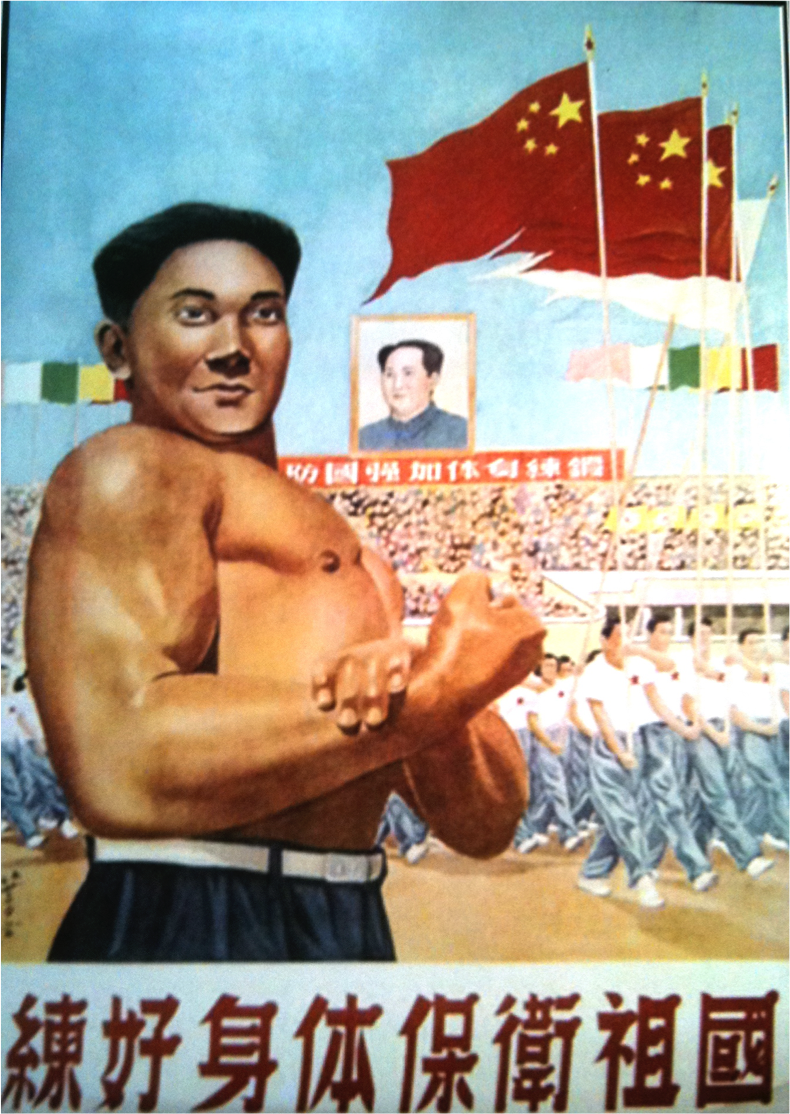
\includegraphics[width = \linewidth,scale=.7]{images/motherlandStrength.png}
   \caption{Strengthen Physique to Defend Motherland (1950)}
   \label{fig:motherlandStrength}
 \end{figure}

 One of the symptoms of the inorganic erection of a sporting infrastructure was that elite sport institutes became separated from education institutions \citep{Brownell2008}.  The widening gap between education and sport in China became the subject of public scrutiny in the early 1980s, but China's sporting success on an international stage during this period delayed policy response.  The PRC won a total of 32 medals at the 1984 Los Angeles Olympics---its first official appearance at the Olympics since it boycotted the games in 1952 due to a dispute with the Republic of China (now Chinese Taipei) over the use of ``China.''  Importantly, 15 of these 32 medals were gold, and this powerful display of strength on the international stage was an enormous moment for modern Chinese nationalism in the reform era \citep{Brownell2008}.  When China produced a much less impressive performance in the summer Seoul Olympics in 1988, winning only 5 gold medals (and a total of 28), latent public criticism of way in which reform era sport had become isolated from society readily surfaced and a ``crisis in Chinese sports'' was declared \citep[199]{Brownell1995}.  Amidst broader social anxieties concerning not only the alarming quantity of the Chinese population (\textit{renkou guoduo} 人口过多), but also the problem of population \textit{quality} (\textit{renkou suzhi} 人口素质), the athlete in China was problematised as lacking sufficient ``cultural quality'' (\textit{wenhua suzhi} 文化素质) in accordance with his or her elevated social status as a ``representative'' (\textit{daibiao} 代表) of the Chinese nation on an ever-expanding international stage (General Administration of Sport 2009a; Brownell 1995: 95).

 In response to this public crisis, in 1989 the Sports Commission adopted a policy modelled on the US college sports system, of ``combining sport and education'' (\textit{tijiao jiehe} 体教结合).  In an attempt to move away from a reliance on sport boarding schools and full-time sports training centres for the development of athletic talent, ``high level sport programs'' (\textit{gaoji tiyu xiangmu} 高级体育项目) were embedded within existing stand alone high schools and universities so as to ensure the ``all-round development''(\textit{quanmian fazhan} 全面发展) of the athlete \citep[203]{Brownell1995}.  As part of an emphasis on a broader range of sports and their perceived potential to facilitate community engagement, international relations, as well as commercial opportunities, various sports programs, including many non-Olympic sports such as rugby (at the time), were inducted into the Chinese sports system for the first time\citep[70]{Knuttgen1990}.  As I explain below, China's first rugby program was a high level sports program, embedded at the Chinese Agricultural University in Beijing in 1990.

 While China has experienced widespread social and economic transformation since the death of Mao in 1976, and while the sport system in particular has experienced numerous waves of policy reform,  the core organisation and the logic of the Chinese sport systems remains largely in tact.  Sports like football and basketball have matured as standalone enterprises with supporting market-based consumer industries, but most other sports in China (i.e., all other Olympic events, including rugby) exist primarily due to the support of the enormous state-sponsored sport system.  Whereas the commercial basketball and football industries might offer a small percentage of prospective athletes incentives of fame and fortune, the benefits of a state-sponsored sports programs like rugby are more modest.  Chinese youth either gravitate or are ushered by their parents towards sporting careers primarily due to potential life-course opportunities such as access to tertiary education and post-athletic career employment.

 Thus, the professional athlete in China occupies a unique position, as both a symbolic representative of Chinese nationalism, as well as the target of various incentives pertaining to life-course opportunities of education and employment.  American cultural anthropologist Susan Brownell, in her monograph ``Training the Body for China'' (1995), was the first to provide a comprehensive development of the subjectivity of Chinese athletes in the (post-Mao) reform era in China.  In reference to the unprecedented success of the Chinese women's volleyball team in the 1980s, including winning China's first ever gold medal in a team event at the LA Olympics in 1984, Brownell explains how elite level sport functioned as a crucial symbolic practice for China in the process of re-joining the world (1995: 86).  As a participant in the sports system as a student-athlete herself, Brownell draws on first-hand ethnographic experience of training and existing as subject to the state-administered ``microtechniques of power'' \citep[citing][]{Foucault1977} designed to cultivate athletes in post-Mao China.  This unique empirical contribution serves to situate the athlete in China between tensions and shifts of an ever-transforming social terrain structured by contradictory forces of top-down state control and the emerging logic of the free market.

 Despite valorisation of the athlete as part of the proletarian revolution during the Mao era (see Section ~\ref{sect:sportPRC}), and some celebration of the nation's top athletes during the post-Mao reform era, a career as a professional athlete remains far from highly desirable or coveted in China, at least not by urban elites.  It is popularly understood that becoming an athlete in China entails sacrificing one's youth (\textit{qing chun} 青春); athletes train incredibly hard and are forced to endure bitterness (\textit{chiku nailao} 吃苦奶酪. It is commonly understood that for women in particular, the physiological demands of being an athlete (weights training, training outside, training during one's menstrual cycle) can threaten one's femininity and fertility, thus harming marriage prospects \citep{Brownwell1995}.  Although recent commercial growth of the sport industry in China has supported the rise and valorisation of ``super star'' athletes in Chinese sport, such as NBA athlete Yao Ming, or 110m hurdles Olympic Champion Liu Xiang, for most wealthy and educated urban Chinese families, the prospect of becoming an athlete does not compare to other life-course trajectories such as pursuing education.  The history of separation between the competitive sport system and the education system is also a factor in discouraging Chinese youth and their families from pursuing sport if it threatens other more attractive life course possibilities within mainstream education institutions.

 Since Brownell's seminal work, very little ethnographic research into the experience of athletes in China has been published \citep[but see][]{Brownell2000,Brownell2008}.  In the more than 20 years since Brownell's ethnographic work was conducted in China, processes of expansion of the market-based economy and political reform have transformed the identity of the athlete in contemporary China, including the nature of incentives and choices available \citep{Taylor2010}.  Yet, professional sport programs like the rugby program at the Institute, remain as attractive possibilities for the pursuit of life-course opportunities.  Generally speaking, athletes rarely gravitate to rugby programs in China looking for fame or fortune, or as part of a perceived duty to be a symbolic ``representative.''  However, as I explain in more depth below, adherence to rugby does appear to generate strong perceptions of belonging and social identity.

 \subsection{Rugby in China\label{sect:rugbyInChina}}
 %\myparagraph{Rugby as an university level amateur sport (1990-2009)}
 Although reportedly existing in China within colonial and expatriate circles for more than a century \citep[210]{Reason1979}, and as a modified military exercise as early as the 1930s \citep[135]{Morris2004}, rugby was a late entrant into the Chinese sport system, established as a ``high level sport program'' at  Chinese Agricultural University in 1990.  The advent of rugby in China was thus part of the process of combining sport and education of Chinese sport initiated in the late 1980s.

 The program was originally made up of existing CAU students who expressed interest in the novel activity, but by its second year, the program earned status as a High Level Sport Program and was subsequently advertised to student-athletes across the country \citep[2]{Xu2010}.  Between 1990 and 2009, rugby programs based on this original CAU model were established within over 30 regular universities and specialist sports colleges in cities throughout China.  In addition to these programs, a number of social rugby clubs (\textit{shehui julebu} 社会俱乐部; organisations completely independent of the state sports system) began to form in major cities with high expat populations (e.g., Shanghai, Beijing, Chengdu, Qingdao).

 For the first 20 years of its existence in China, Rugby was part of a large collection of ``cold gate'' sports in China, which had a relatively small participation base compared to other interactive team sports like basketball or football.  The Chinese Rugby Football Association (CRFA) was established in 1997, and both the men and women's national teams, made up of players predominantly from CAU, but also from other well-established programs based at the Shanghai Sports University, Shenyang Sports College, and the People's Liberation Army Sports College. China consistently competes against other nations in the Asia Pacific region (most notably in the Asian Games and the East Asian Games), and is also occasionally involved in top-tier international tournaments such as the International Hong Kong Sevens.

 %\myparagraph{Rugby in China 2010 - 2013 \label{sect:rugbyinChina}}
 Accrual of Olympic status in 2009 transformed rugby almost overnight from its former position as an amateur sport played at university level by a handful of universities.  As an immediate consequence, in 2010 rugby (in its seven-a-side version of rugby sevens) was included as one of 33 events to be held at the 2013 National Games in the city of Shenyang.  This decision spurred provinces to set up professional rugby programs at provincial sports institutes, to compete at the National Games in 2013.  Ten of China's collection of 32 provinces and municipalities that participate in the National Games have full time men's and women's rugby programs.  For Olympic sports in China, results in the National Games (\textit{quanguo yundonghui} 全国运动会) decide the amount of funding a province and its constituent sporting institutes and programs receive.  As such, the National Games are the most important measure of success for athletes, coaches, and administrators in the competitive sports system \citep{Hong2002}.

 When rugby union was officially inducted into the state sponsored sports system in 2010, a total of five full time Men's (Beijing, Shandong, People's Liberation Army (PLA), Liaoning, and Shanghai) and six Women's (Beijing, Shandong, Anhui, Liaoning, Shanghai, and Jiangsu) provincial programs were immediately established, which signalling an intention by these provinces to invest in the sport for the long term.  With the establishment of professional provincial rugby programs catering for tertiary aged athletes (17 years and above) already established, these provinces could subsequently initiate the establishment of city level rugby programs catering for high school aged athletes (10---16 years).  In this way, a previously non-existent development pathway for athletes, coaches, and officials began to emerge in provinces interested in investing in the sport.

 In addition to these full-time provincial programs, three part-time men's (Inner Mongolia, Heilongjiang, and Xinjiang) and two part-time women's (Sichuan and Xingjiang) programs were established, in which these provinces temporarily employed rugby athletes from university programs. The special administrative region of Hong Kong also fielded both a Men's and a Women's side, bringing the total of Men's and Women's teams eligible to compete in the National Games to nine and ten, respectively.

 \subsubsection{The National Games 2013\label{sect:fallFromGrace}}
 Two provinces in particular identified an opportunity to achieve a favourable result at the National Games by heavily investing in this debutant sport in 2010.  The Beijing men's and women's programs (based at the Institute) managed to attract a large amount of China's existing rugby talent from where it was previously based at the CAU.  Importantly, among Beijing's recruits was the unofficially touted ``Boss''  (\textit{Laoda} 老大) of Chinese rugby, Chinese national coach Zheng Hongjun.  Meanwhile, Shandong province, a traditional powerhouse in other provincial sports, succeeded in attracting the majority of the remaining rugby talent.  The pull to Shandong was strong for a large majority of rugby players in China at the time, many of which were originally from Shandong.  Importantly, the talent transferred to Shandong province also included coaching staff, namely Zheng Hongjun's student and soon to be rival, former Chinese Women's Team coach, Lu Xiaohui.  Besides Beijing and Shandong, Jiangsu and Anhui province were strong contenders for the Women's gold medal, while the People's Liberation Army (PLA) and Hong Kong in particular were strong contenders for top spot in the men's competition.

 Beijing's results in the two years leading into the 2013 national games were strongest overall across the men's and women's teams.   However, the traditionally strong Hong Kong men's and women's teams had only occasionally participated in these tournaments due to conflicting international tournaments.  In the semi-finals of the National Games, held in Shenyang at the beginning of September 2013, the Beijing men came up against Hong Kong, while the Shandong men played off against the PLA.  Beijing lost to their stronger and more favoured opponents, and Shandong beat the PLA.  Meanwhile in the women's tournament, both Beijing and Shandong advanced to the final without faltering.  The stage was set: the traditional favourites, Beijing, led by the reining Boss of Chinese rugby, would face Shandong---the underdogs---lead by the Boss's cunning apprentice come challenger.

 The men's final was played first, and in somewhat of an upset, Shandong edged out Hong Kong to win the gold medal by one try (one five-point score or ``touch down'').  In the women's final, scores were level until early in the 2nd half when Shandong went ahead by two tries to nil.  At that point, the Beijing women's team, allegedly under instruction from their coach Zheng Hongjun, suddenly stopped playing.  After being asked by the referee and match officials to continue, the Beijing athletes stood firm and refused to play on, forming a huddle on their side of half-way in the middle of the field. Shandong had no choice but to continue to play out the rest of the 2nd half, running in try after try, until the final score at full time was a farcical 71-0 \citep{Sina2013}.  Shandong was declared victorious, while Beijing called foul play, claiming that the Spanish referee had been unfairly adjudicating the match in Shandong's favour.  The details and dramas of this now well-known story in China's sporting history, known as ``The 2013 National Games Match Strike Scandal'' (13年全运会巴塞门), require more extensive development in a format beyond the scope of this particular thesis.  Suffice to say, the repercussions of this incident for the Beijing provincial rugby program were extremely costly.

 \subsection{The Temple of the God of Agriculture Sports Institute}
 The rugby match-striking-gate of 2013 led to a sudden fall from grace for the Beijing rugby programs.  Between 2010 and 2013 (in the lead up to the the National Games), the Institute Leadership---excited about the prospect of unprecedented national-level success---immediately elevated the men's and women's rugby programs to top-priority status.  Rugby received unrivalled institutional and financial support in the hope that both teams would be crowned National champions---what would have been the Institute's first National Games gold medals since 2004.  During this period, the rugby program attracted a high profile commercial sponsorship deal from Beijing Capital Steel(北京首钢), which enabled the Institute to invest in a team of foreign coaches from New Zealand to come to Beijing on a periodic basis to consult on training and preparation. Both teams also travelled twice to New Zealand for two three-month stints of off-season training and competitions.  Between 2010-2013, the rugby team lived in the Institute's best available accommodation, and ate their meals at the Institute's highest level canteen, reserved for National-level champions.  Right up until the National Games in 2013, the men's and women's teams had met the high expectations set for them, winning all but one of seven national tournaments each.  All indications were positive for Beijing to take home two gold medals.  However, as explained above, the National Games in Shenyang in September 2013 did not transpire as Beijing would have hoped.

 In the end, Beijing came away with one bronze medal (men's team) and one face-destroying disqualification for the women (official review of match referee performance found no evidence of clear foul adjudication).  During my time at the institute, assistant coach of the Beijing men's team, Shi Yan, told me quietly one evening that the Beijing women's rugby team was the first Beijing team in the 48-year history of the National Games not to receive the ``medal for civilised spirit''  (awarded by the Beijing Mayor to all Beijing representatives in the National Games).  All rugby coaches and many senior athletes of the 2013 National Games campaign left the Institute immediately after the match-strike-gate, either to retirement or to continue playing at other provincial programs.  The rugby program at the Institute was all but abandoned at the end of 2013, and remaining athletes from both men's and women's teams were told to take a break for an undetermined length of time.

 \myparagraph{Rugby at the Institute after 2013}
 It wasn't until April 2014, after the dust had settled on the embarrassment of the women's program's widely publicised disqualification, that the men's program was resurrected with the appointment of a new head coach.  The women's program lay dormant for another full year until it was resurrected just in time for preparations for the 2017 National Games. Former Chinese rugby  representative and CAU coach Zhu Peihou was appointed as new head coach of the men's team.  The junior athletes from the previous National Games cycle were recalled back to the Institute to resume training, and coach Zhu was charged with finding new talent to fill the ranks of the team.

 The Beijing men's team endured a series of mediocre performances during the 2014 and 2015 seasons, and clearly lacked experience, talent, and institutional support from the Institute.  A handful of senior athletes who had played in the era of the 2013 National Games remained, and two in particular, Han Xiaolong and Lu Peng were promoted to a transitional athlete-coach status. Unlike Women's assistant coach and former athlete Wang Chongyi, however, both Han and Lu were originally from Shandong province and so did not automatically have Beijing residency required to make them eligible for full time employment at the Institute.  As such, their future place at the Institute was uncertain, and as I found out from both during the course of my ethnographic research, their ability to stay at the Institute would depend on the result the team could achieve at the 2017 National Games: a medal at the National Games would qualify them for a fast-tracked and Institute-sponsored application for Beijing residency application.\footnote{China's infamously rigid residency (\textit{``Hukou''} 户口) system means that only individuals with Beijing residency can hold permanent employment roles at government institutions such as the Institute (\textit{shiye danwei} 事业单位).  Chinese citizens born outside of Beijing can become Beijing residents if offered employment, but due to Beijing's swelling population, the eligibility criteria for this process of naturalisation has become more and more stringent, and fewer and fewer applications are successfully processed, particularly in industries like sport.}

 Despite being only a shell of its former glory, the rugby program at the Institute nonetheless offered attractive incentives to prospective athletes.  The difficulties of Han and Lu in gaining Beijing residency made it clear to more junior athletes that there was little promise of a passage to official Beijing residency or full-time employment at the Institute.  However, the program did offer a much more realistic opportunity of attending the Beijing Sports University (BSU)---considered to be the country's most prestigious sports universities and one of China's select ``big brand universities'' (\textit{mingpai daxue} 民牌大学).  The mass exodus of experienced senior athletes from the rugby program meant that junior athletes from the pre-2013 era were now in a position to represent Beijing at a national level, and in so doing attain the official athletic standard of a ``Master Sportsperson'' (\textit{yundong jianjiang} 运动健将).  A Master Sportsperson was automatically eligibility to attend BSU through its arrangement with the Institute.  It was in this context that I entered the Institute and began ethnographic research.

 %Professional sport program: incentives.

 %Nonetheless,


 %The women's program was inactive for a full two years after 2013, and was only just starting to re-activate after I arrived, in November 2015.  Thus, rugby was resurrected at the Institute, but was no longer in centre stage.


 \subsection{Method}
 The empirical research analysed in this thesis consists of an  in-depth ethnographic study of the Beijing men's rugby team ($n = 26$), and two field experimental studies: one survey study during a National rugby tournament ($n = 174, male = 91$), and a controlled field experiment ($n = 58, male = 31$).  The methodological details of the field experimental studies are introduced in the introductory sections to each study (see Chapters ~\ref{chap:tournamentSurvey} and ~\ref{chap:trainingExperiment}).  Below I outline the method through which I collected ethnographic data, with further detail included in Appendix~\ref{app3:researchSetting}.

 \subsubsection{Ethnography}
 I conducted a three stretches of participant observation at the Institute, totalling ten months between September 2015 and September 2017 (1st stretch = 7 months, 2nd stretch = 2 months, 3rd stretch = 1 month).  During these stretches, I lived full-time at the Institute and attended (and often participated in, predominantly as coach) training sessions, team meetings, meals, and any other activities relevant to the rugby program.  In addition to participant observation, I also conducted semi-structured interviews and administered a series of informal surveys following training and at different intervals throughout my time at the Institute.  I recorded field notes using Evernote (Version 7.4.1), an electronic note taking software that was synchronised across my mobile and personal computer devices.

 The institute was home to both a men's and women's rugby team, each with usually 20-30 athletes and 2-4 coaches per team.  However, for reasons outlined above, when I arrived to conduct research only the men's team was in active training.  As such, I dedicated my ethnographic research to the Beijing men's team only.  I analysed data on a total of 26 athletes ($age = 20.96, range = 17-27, SD = 3.17$)   Athletes were included in data analysis if they participated in 1) a semi-structured interview, 2) at least one informal survey relating to experiences of rugby training and group membership, and 3) at least two months of training at the Institute. Table ~\ref{tab:ethnoDescriptivesTable} for a summary of athlete attributes, which will be discussed at more length below.  I sought permission to conduct research at the Institute was from relevant authorities and directly from athletes at the beginning of the first research period in September 2015.

 % latex table generated in R 3.5.0 by xtable 1.8-2 package
% Wed Jun 20 16:44:16 2018
\begin{table}[ht]
\centering
\begin{tabular}{ll}
  \hline
row & Overall \\ 
  \hline
n &    26 \\ 
  Age (mean (sd)) & 20.96 (3.17) \\ 
  ResearchCategory = Senior (\%) &    10 (38.5)  \\ 
  TrainingAge (mean (sd)) &  3.34 (2.02) \\ 
  YearsInTeam (mean (sd)) &  2.59 (1.80) \\ 
  AthleteStatus (\%) &     \\ 
     Master Sportsperson &    10 (47.6)  \\ 
     Level 1 &     6 (28.6)  \\ 
     Level 2 &     5 (23.8)  \\ 
  ContractStatus (\%) &     \\ 
     Permanent Employee &     1 ( 3.8)  \\ 
     Full Time Contract &     7 (26.9)  \\ 
     Training Contract &     5 (19.2)  \\ 
     Student Contract &     6 (23.1)  \\ 
     Trial &     7 (26.9)  \\ 
  EducationLevel (\%) &     \\ 
     Graduate &     1 ( 3.8)  \\ 
     Undergraduate &    12 (46.2)  \\ 
     High School &    10 (38.5)  \\ 
     Middle School &     3 (11.5)  \\ 
  HomeProvince (\%) &     \\ 
     Shandong &    11 (42.3)  \\ 
     Beijing &     6 (23.1)  \\ 
     Jiangsu &     3 (11.5)  \\ 
     Liaoning &     2 ( 7.7)  \\ 
     Hebei &     2 ( 7.7)  \\ 
     Heilongjiang &     1 ( 3.8)  \\ 
     Fujian &     1 ( 3.8)  \\ 
  PreviousSport (\%) &     \\ 
     Athletics &    16 (61.5)  \\ 
     None &     8 (30.8)  \\ 
     Basketball &     1 ( 3.8)  \\ 
     Football &     1 ( 3.8)  \\ 
   \hline
\end{tabular}
\caption{Athlete Desciptives (n = 26)} 
\label{tab:ethnoDescriptivesTable}
\end{table}


 In addition to researching athletes, I also engaged coaches, officials, and informants with relevant knowledgeable of rugby and sport in China. Data collected on these individuals were not included in the main analysis, but provided valuable contextual information.
 All my interactions with athletes took place in Modern Standard Chinese (Mandarin or \textit{putonghua} 普通话).  To record these interactions, I would either interrupt conversation to ask permission to start the audio recording device within the Evernote application on my mobile phone.  Alternatively, in the case of shorter or unplanned interactions that were relevant to my research questions,  I transcribed shorter conversations using my notebook or phone immediately following these interactions.  Every week or fortnight I collated, summarised, and organised these notes by date and by theme.  Interview recordings were transcribed into written Chinese by a native Chinese speaking research assistant using a ``verbatim'' method \citep[i.e., including an account of all verbal and important nonverbal (coughs, pauses, etc.) utterances, see][269-70]{Poland2003}.  I analysed interviews in Chinese and only translated into English data extracts that were included in the main analysis of this thesis.

 I collated all ethnographic data into a corpus that was subjected to a process of ``thematic analysis'' \citep{Braun2006}. I identified themes that captured important information about the data in relation to a research question or hypothesis.  I attempted to identify themes on both explicit and implicit levels of the data \citep{Boyatzis1998}.\footnote{The story of Sun Hongwei (see the opening vignette of Chapter~\ref{sect:SHW}) serves as a good example of the contrast between implicit and explicit levels of data.  In our interview, Hongwei was able to articulate many conceptions relating to joint action and social bonding, all of which were recorded as explicit declarations.  At the same time, I observed in training that Hongwei, while fluent in his declarations in interview, was far form fluent in his more embodied declarations on the field.  The combination of implicit and explicit data offered points of contrast and comparison that were fruitful for richer analysis.}  Following a process of theme rationalisation and reduction,
 relevant data (selected from the original corpus) were reorganised in a matrix in which themes formed the columns, participants formed the rows, and selected evidence formed the cells (see Appendix~\ref{app3:ethnoAnalysis} for a full explanation of method).


 \myparagraph{The life of an athlete in the Beijing rugby team}
 The Beijing men's rugby team competed against other provinces in five national tournaments held in different locations across the country every year between March and September.  The period in which I conducted my first stretch of ethnographic research (August 2015 --- February 2016), therefore, constituted the off-season and pre-season components of the training year.  Due to cold weather in the north of China during winter and spring, teams from northern China (e.g. Beijing, Liaoniang, and Shandong provinces) often elected to train at other domestic or international training locations depending on amount of program funding available and the training strategy of each program.  In 2015, before an unexpected change in coaching team at the end of December, the head coach of the Beijing Men's team had planned to travel to Yunnan province in early 2016 for one month of altitude training before moving closer to sea-level somewhere in the south of China for one month (February/March).  Following the coaching leadership change, the team did not leave Beijing until after Chinese New Year (25th February). Training during this period was therefore consistently stationed at the Institute in Beijing, and as such subject to occasional disruption due to Beijing's cold winter weather and air pollution.

 All athletes lived and trained 6 days a week at the Institute, and would occasionally attend university or high school classes as part of their ongoing education commitments.  Below is a table of a typical weekly training schedule (see Figure ~\ref{tab:trainingSchedule}). A typical week consisted of 10 two and a half hour ($\approx 150 minute$) training sessions, seven of which were on-field rugby sessions, three of which were strength and conditioning sessions (not involving a rugby-specific skills).  In addition, two one hour evening skills sessions were also allocated for junior athletes to hone their basic skills of passing, catching, and game-play.  Athletes lived full-time on campus in the Institute's dormitory accommodation (usually 3 athletes per room), and were permitted to take overnight leave on the weekend after the conclusion of Saturday morning training.  Athletes from Beijing or with family in Beijing would usually take this leave, while the remaining athletes would spend weekends at the Institute.  Generally speaking, the rugby program would break at the end of the national season in September for two weeks, and occasionally around Chinese New Year for 7-10 days, unless New Year interrupts pre-season training plans, in which case training would continue in spite of this national holiday.

 \input{images/trainingScheduleTable}

 \subsubsection{Positionality of the researcher}
 My unique positionality as a researcher requires further consideration, due to the way in which my identity as foreign ``friend of Chinese rugby,'' professional athlete, and authoritative rugby coach may have induced bias in the testimonies and behaviours of my research participants \citep[referred to in experimental psychology as ``demand characteristics''][]{McCambridge2012}.

 My history of interaction with the Chinese rugby community (during previous stretches of study, work, and rugby coaching) meant that I was well known by most Chinese rugby coaches, and many current athletes, particularly older athletes.  Of the 26 athletes whose data I analysed, I had only previously interacted one athlete, Han Xiaolong (the most senior and experienced athlete in the team, Han was a student at CAU when I was based in Beijing in 2008).  Indeed, my established relationships and familiarity within the Chinese rugby community were what enabled unique access to group exercise context in the first place.  However, my status as a ``friend of Chinese rugby'' may have also left me liable to attracting from my participants testimonies and rationales that were in part motivated by their desire to tell me what they thought I wanted to hear \citep{Clifford1986}.  In addition, my position of authority in relation to rugby, owing to previous experience as a professional rugby player in Australia and my authority as occasional coach at the Institute, may have meant that athletes did not freely express their personal attitudes to me in interviews or in surveys.

 Comparisons between China and West commonly featured in my informal and semi-structured interactions with participants.  By and large, athletes with whom I engaged understood that they were engaged in a fundamentally foreign or Western sport, and they would also often treat me---a foreigner with expert knowledge of rugby---as a representative of both the ``West'' and rugby in the West, more specifically.  My specific research aims, questions, and hypotheses meant that I was interested in disentangling the sources or meanings of these generalisations.  Rather, I treated such rationales as evidence of the cultural affordances that athletes employed in order to successfully bridge the gap between our respective subjectivities.

 In addition, while I consider myself professionally fluent in Modern Chinese, my level of proficiency was not at the level of native a native speaker, and it is possible that at times I missed important nuance and detail that could have been relevant to interpretation of data. Further, my own intuitions and values may have influenced the ways in which I judged and inferred significance of certain observations and  events over others.

 Based on these considerations, I aimed to adopt a skeptical, self-reflexive stance when analysing ethnographic data \citep{Lichterman2017}, and attempted where possible to triangulate more explicit or declarative testimonies (e.g. interview data) with more implicit observational data \citep[see, for example:][]{Duffy1987}.
 When briefing research participants, I explained that I was generally interested in researching ``athlete's on-field and off-field experience of rugby.'' I hoped that by limiting the detail associated with my brief, and by promoting the notion of (subjective) experience of adherence to rugby, I would encourage athletes to reflect in more personalised and less generalised or stereotypical ways.



 %\subsubsection{Field experiments}

 %Brief intro and justification?
 %A full introduction to the field experiments of this thesis are described in the introductory sections to each study (see Chapters)





\section{Discussion}















                                                          \end{CJK}
